% IEEE S&P 2027 submission format; requires IEEEtran.cls v1.8b.
\documentclass[conference,compsoc]{IEEEtran}

\usepackage[T1]{fontenc}
\usepackage[utf8]{inputenc}
\usepackage{booktabs}
\usepackage{tabularx}
\usepackage{array}
\usepackage{graphicx}
\usepackage[dvipsnames,table]{xcolor}
\usepackage{tikz}
\usetikzlibrary{arrows.meta,positioning,fit,calc,matrix,shapes.geometric}
\usepackage[hyphens]{url}
\usepackage{hyperref}

\hypersetup{hidelinks,pdfauthor={}}
\newcommand{\scope}{\textsc{Scope}}
\newcommand{\NRR}{\textsc{nr-r}}
\newcommand{\NRA}{\textsc{nr-a}}
\newcommand{\NRV}{\textsc{nr-v}}
\newcommand{\NA}{\textsc{na}}
\newcommand{\evidenceStrong}{\cellcolor{ForestGreen!22}Strong}
\newcommand{\evidenceLimited}{\cellcolor{Goldenrod!24}Limited}
\newcommand{\evidenceNone}{\cellcolor{Gray!18}No verified direct evidence}
\newcolumntype{Y}{>{\raggedright\arraybackslash}X}
% Additive finite-candidate reconciliation; historical snapshots retained.
\newcommand{\FinalN}{60}
\newcommand{\FinalCore}{43}
\newcommand{\FinalA}{15}
\newcommand{\FinalB}{28}
\newcommand{\FinalAdjacent}{17}


\title{SoK: From LLM Inference Side Channels to Agent Workflow Leakage}
\author{}
% Coded-study cutoff: October 8, 2026. Screening provenance updated October 18.
% October 19 source-consistency follow-up: see Appendix Receiver-Contract Support.

\begin{document}
\maketitle

\begin{abstract}
Side-channel results measured at one interface are often relevant to another deployment, but relevance alone does not establish transfer. We systematize \FinalN{} LLM/agent study families using one result record that binds the hidden target, receiver permissions, intervention, attacker procedure, workload and outcomes to a source version. Three deployment cases yield an actionable rule: locate the final target-bearing emitter, determine whether cover reaches action dispatch, and bind adaptation and cost to that same condition. This permits source-local conclusions while identifying the bridge required for a different receiver or mechanism. Upstream padding does not certify a content-aware downstream emitter; transport costs cannot establish task-preserving dummy actions; a component microcost cannot price another cache or a full service. We distinguish direct instances from extensions and background, with explicit source-deletion sensitivity. A short public-archive example shows a predictive sequence increment under archive-receiver ordering; task-independent identity and ordinary-website capture remain unresolved. A separate workflow comparison is negative for SCOPE against an information-matched structured checklist. The contribution is the source-linked deployment judgments and their conditional permissions, rather than a new attack or demonstrated review advantage. Incomplete acquisition, unresolved run bindings and absent independent researcher adjudication constrain the synthesis.
\end{abstract}

\section{Introduction}\label{sec:introduction}
Encryption conceals content but need not conceal execution. LLM services produce token streams, cache hit/miss timing and shared-resource activity; agents add destinations, tool exchanges and website actions. A receiving website, a passive network observer and an active API client see different projections \cite{weiss2024prompt,promptpeek2025,earlybird2025,agentprint2025,uitraces2026,jeong2026wra}. The practical question is which deployment decision a favorable defense result actually supports.

A designer may find relevant results without finding an answer to that decision. NetEcho studies downstream re-emission, Dangol measures transport cover, AHB measures executed mobile humanization, and UI Traces studies classifiers fitted to delayed traces \cite{netecho2025,dangol2026workflow,zhu2026turing,uitraces2026}. Each supplies useful evidence. Their percentages and overheads answer different questions, however: what reaches the receiver, what executes, what task outcome remains, and what component the cost measures. A whole-paper defense label obscures these differences.

\paragraph{Central contribution: result-bound deployment judgments}
We develop three complete cases around choosing the final protected interface, deciding whether cover may execute, and selecting an applicable adaptation result and price. Each names the decision, relevant source results, the judgment after condition binding, and the evidence that permits transfer. The resulting rule is to locate the final target-bearing emitter, trace cover to its execution boundary, and bind inference, objective utility and applicable cost to that condition. It preserves positive local conclusions rather than simply declaring the evidence insufficient.

The individual phenomena are already established by the original papers. Our knowledge product is their cross-paper decision mapping: when to test residual features, when to capture a final hop, and when to measure executed task/policy effects. Verified discard before semantic dispatch removes the direct fake-touch mechanism while leaving possible resource and delay effects. The same tested receiver view permits a local adaptation conclusion; a new view needs a bridge. Component costs remain valid for the component, rather than becoming a full-service ranking. These are conditional permissions, not a new composition theorem or alleged corrections of author errors.

\paragraph{Corpus and outputs}
The October 8, 2026 coded collection contains \FinalN{} families: \FinalCore{} core (\FinalA{} workflow-origin and \FinalB{} inherited-runtime/application) plus \FinalAdjacent{} adjacent. Four core components concern privileged diagnostics. Identity/provenance attribution and human--agent distinction are explicitly separated from confidentiality leakage. One result record unifies the method; SCOPE indexes its target, channel, observer, pipeline and inference goal. The outputs are a source--receiver--intervention matrix, three deployment judgments, an applicable-cost subset, and source-deletion/NR sensitivity. The accompanying evidence package links every family, result, source locator and supported claim.

A compact public-trace worked example illustrates a fixed-view prediction decision under archive-receiver ordering. Its task-matched control is inconclusive and its ordinary-site capture bridge is unverified. The separate workflow test favors the complete structured checklist on its original joint endpoint; it establishes no SCOPE review advantage. Failed pilot and retail outcomes are preserved. Remaining acquisition gaps and absent independent researcher adjudication materially limit the synthesis; the paper does not use the corpus count or AI agreement as substitutes for that evidence.

\begin{figure*}[t]
\centering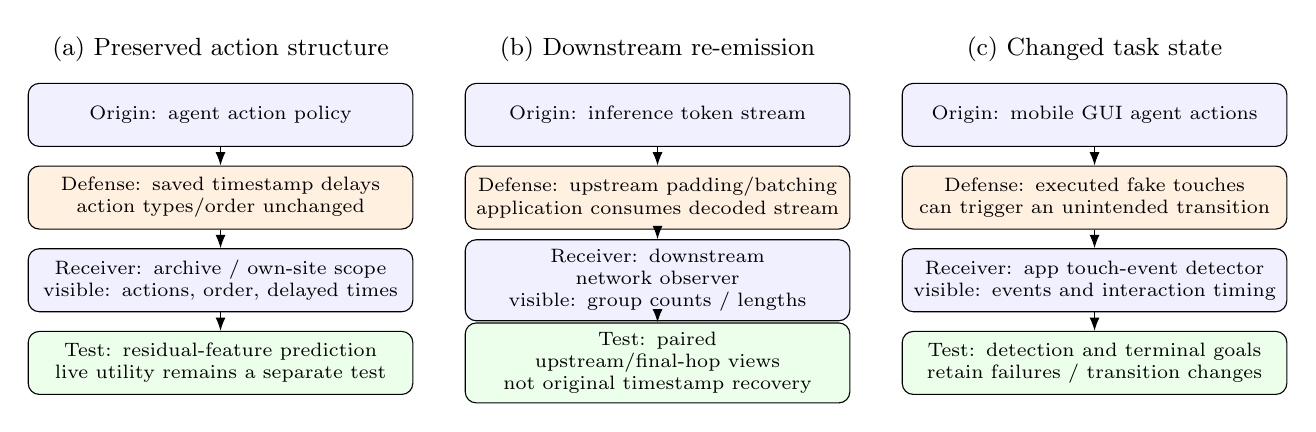
\begin{tikzpicture}[font=\scriptsize,>=Latex]
\tikzset{box/.style={draw,rounded corners,align=center,text width=4.65cm,minimum height=8mm,fill=blue!6},def/.style={box,fill=orange!12},test/.style={box,fill=green!8}}
\foreach \x/\title in {0/{(a) Preserved action structure},5.55/{(b) Downstream re-emission},11.1/{(c) Changed task state}}{
\node[font=\small,anchor=south] at (\x,0.55) {\title};}
\node[box] (a0) at (0,0) {Origin: agent action policy};
\node[def] (a1) at (0,-1.05) {Defense: saved timestamp delays\\action types/order unchanged};
\node[box] (a2) at (0,-2.1) {Receiver: archive / own-site scope\\visible: actions, order, delayed times};
\node[test] (a3) at (0,-3.15) {Test: residual-feature prediction\\live utility remains a separate test};
\node[box] (b0) at (5.55,0) {Origin: inference token stream};
\node[def] (b1) at (5.55,-1.05) {Defense: upstream padding/batching\\application consumes decoded stream};
\node[box] (b2) at (5.55,-2.1) {Receiver: downstream network observer\\visible: group counts / lengths};
\node[test] (b3) at (5.55,-3.15) {Test: paired upstream/final-hop views\\not original timestamp recovery};
\node[box] (c0) at (11.1,0) {Origin: mobile GUI agent actions};
\node[def] (c1) at (11.1,-1.05) {Defense: executed fake touches\\can trigger an unintended transition};
\node[box] (c2) at (11.1,-2.1) {Receiver: app touch-event detector\\visible: events and interaction timing};
\node[test] (c3) at (11.1,-3.15) {Test: detection and terminal goals\\retain failures / transition changes};
\foreach \p in {a,b,c}{\draw[->] (\p0)--(\p1);\draw[->] (\p1)--(\p2);\draw[->] (\p2)--(\p3);}
\end{tikzpicture}

\caption{Three source-bound situations: preserved actions (UI Traces), downstream group/length re-emission (NetEcho), and state-changing executed touches (AHB). Signal path and task-state effect determine different deployment tests.}
\label{fig:system-model}
\end{figure*}

\section{Scope and Review Method}\label{sec:methodology}\label{sec:background}
\subsection{Questions and eligibility}
We ask which hidden targets and observables appear (RQ1), how signal origin relates to receiver permission (RQ2), what establishes feasibility and transfer (RQ3), and which intervention addresses which observable at what cost (RQ4). An agent selects and executes actions using an LLM, tools, memory or orchestration; inherited serving and hardware channels need not be agent-specific.

Core eligibility requires (C1) LLM/agent execution, (C2) a hidden target, (C3) an execution-dependent auxiliary observable rather than ordinary output semantics alone, (C4) specified observation permissions, and (C5) an empirical inference evaluation. A controlled synthetic-state inference can satisfy C5; a proposed mechanism or timing gap alone cannot. Mixed papers qualify through an identifiable component. Table~\ref{tab:boundary-rules} supplies the decision rules.
\begin{table}[t]\centering\footnotesize
\caption{Observable-based eligibility. A hidden target alone does not make a semantic attack a side channel.}\label{tab:boundary-rules}
\begin{tabularx}{\columnwidth}{@{}p{.39\columnwidth}Y@{}}\toprule
Observed input & Decision and required distinction\\\midrule
Length, timing, cache response & Core when measured execution dependence supports hidden-target inference.\\
Own-site actions & Core attribution with site permission; no automatic access to other sites or private tool logs.\\
Reply states the secret & Direct disclosure; adjacent, not auxiliary-channel evidence.\\
Reply style/content identifies a user & Adjacent unless a separately evaluated auxiliary mechanism is established. WildAuth stays a mixed-view comparator.\\
Output-filter membership oracle & Can be core: the filter's execution, not ordinary semantic output inference, mediates the signal.\\
Privileged loop/fault logs & Separate diagnostic component when C1--C5 hold; does not increase confidentiality evidence.\\\bottomrule
\end{tabularx}\end{table}


The final coded collection contains \FinalN{} families available by October 8, 2026: \FinalCore{} core (\FinalA{} workflow-origin, \FinalB{} inherited-runtime/application) and \FinalAdjacent{} adjacent. Four core components concern authorized diagnostics. Other targets include content/property inference, provenance attribution and human/agent distinction; hiddenness alone establishes no confidentiality violation. Families are deduplicated studies; result records distinguish conditions within a study.

The auxiliary-only rule is applied consistently. Coding fingerprints and WildAuth remain adjacent because their evaluated views mix semantic and interaction features; feature importance is not a separately evaluated auxiliary-only attack \cite{ghaleb2026codingfingerprint,wang2026dialogue}. Metric-only fault localization qualifies as a diagnostic component despite operator authorization. ZeroPrint's response differences, endpoint-content fingerprints and StepFinder's mixed view remain adjacent \cite{scheinert2026rca,shao2026zeroprint,leshin2026endpoint,zhu2026stepfinder}.

\subsection{Executable scope and acquisition limits}
Native IEEE/ACM exports, a fixed 40-seed one-hop citation route and exact-title/DOI source lookup form the acquisition routes. Appendix~\ref{app:search} prints the executed queries, fields, dates and export rules. Source versions are merged only with identity evidence. Backward tracing covers 2,237 reference occurrences; forward lookup resolves 38 seeds and returns 24 distinct works. Neither route is recursively exhaustive.

We distinguish the acquired candidate frames from the coded collection. The prepared metadata frame contains 4,753 unique IDs with a recorded exclusion, referral or unresolved disposition. A bounded source reconciliation accounts for 109 overlapping decision rows in four nominated frames (57 follow-ups, six proposals, 22 backward candidates and 24 forward records). A disposition map includes pending material; it is not 109 independent full readings. Recent empirical channels, evaluated interventions, new receivers, prior systematizations and potential counterexamples receive source-review priority.

Broad database coverage remains incomplete: IEEE Q4's 35,743 historical hits were not fully acquired, and Q4b's 847 exports do not establish retained coverage. The dated ACM frame has 13,201 groups, including 883 referrals and 2,950 unresolved routes. The frames overlap and do not constitute a complete PRISMA funnel. Known-paper export yields are reported separately from indexing and field eligibility; they are not recall estimates. These limitations can conceal counterexamples or closer frameworks, not merely distort prevalence. Our conclusions therefore identify the exact result pairs that support them and expose single-source dependence.

\subsection{Coding, adjudication and reproducibility}
The extraction dictionary specifies receiver permissions, auxiliary versus semantic observations, result splitting, execution mode, utility/cost object and source/run binding. Source-scoped \NRR{}, unavailable \NRA{} and unverified \NRV{} remain distinct from replication. Code inspection can establish implementation behavior without authenticating the historical run.

Screening and targeted rechecks are AI-assisted. The 23-case label-blinded exercise has 17/21 agreement among determinate second judgments; the 332-dispute readbacks and separate exclusion audits are reported in Appendix~\ref{app:search}. They neither establish independent researcher coding nor estimate missed eligible studies. The supplied independent-review packets cover central sources, all mitigation families, unresolved defense assertions, boundary decisions and high-risk exclusions; no researcher returns have been received. Consequently, interpretation-sensitive judgments retain this validation limitation.

All \FinalCore{} core families have a scoped intervention disposition. The companion Supplementary Evidence package supplies the 60-family index, 33 result records, 66 utility/cost field positions, source versions/locators, claim links and a fit-free verifier. Table~\ref{tab:result-lineage} gives a complete chain in the paper itself. Appendix~\ref{app:claim-sensitivity} tests source deletion and unresolved bindings. The package can be reviewed as an accompanying file; public hosting and independent researcher validation are not claimed.

\section{Result Records and Comparison Rules}\label{sec:scope}
The unit of comparison is one evaluated condition, rather than a paper or a headline score. A result record binds a source version and locator to its target, receiver, intervention, attacker procedure, workload and outcomes (Table~\ref{tab:result-record}). A family can contribute several records when it reports different execution modes, protected views or cost components. This is why a valid result can answer one deployment question while leaving another unresolved.
\begin{table}[t]\centering\footnotesize
\caption{A single result record. Only fields relevant to the requested comparison must align; unavailable required fields remain unresolved.}\label{tab:result-record}
\begin{tabularx}{\columnwidth}{@{}p{.24\columnwidth}Y@{}}\toprule
Record field & Required meaning\\\midrule
Source & Family/result ID, version, source locator, reading scope and hash.\\
Target & Hidden property, inference goal and protection relation: confidentiality, attribution, human/agent distinction or authorized diagnosis.\\
Receiver & Actual permission and released representation, including session/document linkage and any auxiliary inputs.\\
Intervention & Where protection ends; whether edits affect stored traces, transmission or executed actions.\\
Attacker & Fit/calibration condition, test population, training access and adaptation budget.\\
Workload & Task, system, topology/hardware and grouping/holdout.\\
Outcomes & Inference metric/denominator; objective or proxy utility; applicable cost object; uncertainty and field states.\\\bottomrule
\end{tabularx}\end{table}


\paragraph{One record, two indexing aids}
\scope{} indexes the record's Secret/target, Channel, Observer, Pipeline and Exploitation goal. The Evidence Plane is the record's source and evaluation columns, not a second taxonomy or an evidence score. Pipeline indices distinguish hardware (P1), serving (P2), transport (P3), application/API (P4), orchestration (P5), tools/MCP (P6), environment (P7) and multi-agent communication (P8). A generating layer and a receiving layer can differ. Permission, activity, calibration access and protection relation are separate fields: an authorized fault-localization component is not thereby a confidentiality attack, and an attribution label is not automatically a protected secret.

\paragraph{Three comparison outcomes}
A \emph{compatible} comparison has evidence for the fields needed by the requested inference. An \emph{incompatible} comparison has a positively established mismatch, such as token payload versus wire bytes or stored timestamps versus executed actions. An \emph{unresolved} comparison lacks a necessary binding or transfer test. Only the affected inference is withheld: an unreported task endpoint does not invalidate a measured bandwidth cost. Table~\ref{tab:comparison-contracts} applies these outcomes to descriptive comparison, paired effects and deployment transfer.
\begin{table}[t]\centering\footnotesize
\caption{Comparison rules. A known mismatch and a missing binding have different consequences.}\label{tab:comparison-contracts}
\begin{tabularx}{\columnwidth}{@{}p{.28\columnwidth}Y@{}}\toprule
Requirement & Condition and resulting license\\\midrule
Descriptive comparison & Align target, receiver permission, metric meaning and cost object. Different systems may be described together; token payload and wire bytes cannot be ranked as the same cost.\\
Paired effect & Compare the same defended test population and outcome. A known population mismatch makes that subtraction incompatible; an unverified fit binding leaves the effect unresolved.\\
Deployment transfer & Establish a bridge for the changed receiver, intervention, workload, topology or hardware. A demonstrated violation blocks the proposed transfer; an untested bridge leaves it unresolved. Permit only the range and endpoints actually covered.\\\bottomrule
\end{tabularx}\end{table}


\paragraph{Missingness and adaptation}
\NRR{} records a quantity unreported within the inspected source scope; \NRA{} records unavailable material; \NRV{} records an unverified field, version or run binding; \NA{} records inapplicability. A missing field gives an unresolved judgment, not an observed mismatch. Fitting on protected data (D1) and comparing clean- versus protected-trained procedures on the same defended test population (D2) are separate entries in the attacker column. Neither alone establishes that the observer can obtain the labeled data or afford the fitting budget.

\paragraph{A complete traceable example}
The chain below connects a family, a result, the inspected source and the deployment judgment. The same identifiers join the supplied family index, result ledger and claim links; full source hashes and reading scopes remain in the companion evidence package.
\begin{table}[t]\centering\footnotesize
\caption{Filled record and its licensed judgment. Values are source-reported; no cross-mode effect is computed.}\label{tab:result-lineage}
\begin{tabularx}{\columnwidth}{@{}p{.24\columnwidth}Y@{}}\toprule
Join key / field & Entry\\\midrule
Family / result & \texttt{dangol2026workflow} / \texttt{DANGOL-livebinding}.\\
Version / locator & arXiv:2606.07150v3, \S9.7, OHTTP paragraph after Table~5 \cite{dangol2026workflow}.\\
Target / view & Workflow classification from the evaluated live OHTTP/A2A traffic view; not GUI-state observation.\\
Intervention & Live fixed-rate cover with fresh per-session identifiers, distinct from transformed stored captures.\\
Workload / testbed & Workflow classes with client, relay, gateway and agent co-located on one loopback host.\\
Outcome / cost & Accuracy 0.30; about 13$\times$ bytes and 11$\times$ latency in that condition.\\
Unresolved fields & Objective terminal task utility \NRR{}; precise paired live-refit comparison \NRV{}.\\
Licensed judgment & These costs describe this live protocol condition. They neither price dummy GUI actions nor prove task preservation. A matched objective endpoint is needed for the latter.\\\bottomrule
\end{tabularx}\end{table}


\paragraph{Scope of the method claim}
A complete structured checklist can express these same checks. The separate model-assisted comparison favors that checklist on its original joint endpoint (Appendix~\ref{app:scope-workflow-boundary}). We use \scope{} to organize the resulting knowledge; improved review accuracy, efficiency and human usability are unestablished.

\section{Corpus Map and Nearest Prior Work}\label{sec:corpus-map}
\subsection{Origins and receiving projections}
Ring B signals arise from inference, serving and application mechanisms inherited by agents; Ring A signals arise from orchestration, tools, browser actions and multi-agent execution. Origin is not receiver location. Table~\ref{tab:origin-receiver-map} counts source-coded origins within observable/permission profiles, including diagnostic components as such. Table~\ref{tab:receiver-intervention-matrix} maps load-bearing result paths; the supplemental family index retains all versions and additional views.
\begin{table*}[t]\centering\footnotesize
\caption{Primary observable/receiver profile $\times$ signal origin in the \FinalCore{} core families. Each family occupies one profile row but may have multiple origins; cells count families, not results. Extra observer views remain in the ledger. Zeros are not field-wide gaps.}\label{tab:origin-receiver-map}
\begin{tabularx}{\textwidth}{@{}YrrrrrrrY@{}}\toprule
Observable / receiving permission & P1 & P2 & P4 & P5 & P6 & P7 & P8 & Representative source\\\midrule
Flow/destination & 0 & 8 & 0 & 5 & 1 & 2 & 2 & AgentPrint; WRA; NetEcho \\
Own-site actions/attributes & 0 & 0 & 0 & 5 & 0 & 5 & 0 & UI Traces; FP-Agent \\
API duration/cache/oracle & 0 & 12 & 0 & 0 & 0 & 0 & 0 & Early Bird; LeakyLMs \\
Resource/physical & 10 & 3 & 0 & 1 & 0 & 0 & 0 & TDXRay; ClawGuard; LLM RCA (diagnostics) \\
Trajectory/procedure/log & 0 & 0 & 1 & 4 & 2 & 0 & 0 & SIGLEAK; cycle detection (diagnostic) \\
\bottomrule\end{tabularx}
\par\smallskip\raggedright\footnotesize P1 hardware; P2 serving; P4 application/API; P5 orchestration; P6 tools; P7 environment; P8 multi-agent. P3 is a receiving layer here, not a coded signal origin. Composite origins are multi-label descriptions, not independent channels. Privileged logs and physical diagnostic receivers are not ordinary website capabilities.
\end{table*}


\paragraph{Inherited channels}
Weiss reconstructs candidate text from encrypted length sequences; NetEcho's semantic information recovery is not exact-text recovery \cite{weiss2024prompt,netecho2025}. Whisper Leak classifies topics from traffic, while Time Will Tell uses aggregate completion time \cite{whisperleak2025,timewilltell2024}. Different targets and metrics prevent treating their percentages as attack strength. Chosen-request cache attacks use shared-state timing oracles; local CPU-cache and GPU interference attacks require different permissions \cite{promptpeek2025,earlybird2025,inputsnatch2024,spliceleak2026,spillbeans2025,gu2026behindbars}. LeakyLMs' architecture branch requires same-GPU-class calibration; KVGov separates hardware timing, simulated inference/defense and analytic controls \cite{majidi2026leakylms,addagada2026kvgov}.

\paragraph{Workflow channels and target relations}
AgentPrint, the Web and Research Agents (WRA) study, and the traffic benchmark infer identities, activities or traits through flow/destination structure. UI Traces and FP-Agent use own-site behavior or browser attributes \cite{agentprint2025,jeong2026wra,pouryousef2026traffic,uitraces2026,wang2026fpagent}. URL and domain views are distinct; passive encrypted observation does not reveal endpoint method semantics. AgentTell's probe site, PlanTwin's planner and SICC's authorized recipient occupy still different projections \cite{shahriar2026agenttell,yu2026plantwin,xu2026sicc}.

The \FinalCore{} core families include 39 non-diagnostic components and four privileged diagnostics (ClawGuard, cycle detection, LumiMAS and LLM-serving fault localization). The latter uses 120 controlled fault injections and supplied onset times, not a low-permission privacy observer \cite{scheinert2026rca}. Model/human attribution is not by itself a confidentiality violation. Coding fingerprints, WildAuth, SymDiag, ZeroPrint, endpoint fingerprints and StepFinder are adjacent semantic-boundary comparisons. AgentDAM is a background data-minimization benchmark, not auxiliary inference \cite{ghaleb2026codingfingerprint,wang2026dialogue,cui2026symdiag,agentdam2025}. The target-relation ledger records these differences without converting every hidden property into a protected secret.

\subsection{What earlier systematizations already establish}
Cross-layer composition and inference-to-agent transfer are prior insights, not our discoveries. Banerjee et al. organize compound-system attacks by cross-layer mechanisms and MITRE threat models; Forough et al. v2 distinguish transferable inference protection from memory/action/coordination requirements under confidential computing \cite{banerjee2024compound,forough2026secrets}. Both are background prior-systematization sources, not C5 attack families.

A concrete shared precursor is Debenedetti's auxiliary-component privacy channel, also cited by Banerjee: its lesson about composition is already established. Our narrower increment concerns intervention placement. NetEcho identifies a downstream view that must be checked after upstream protection; Dangol/AHB distinguish transport cover from cover that executes and changes the task. Together they specify two different reasons why an apparently suitable timing defense needs another measurement, and the conditions under which each concern would disappear. Likewise, Forough already distinguishes a trusted execution environment (TEE) boundary from side-channel resistance; our Early Bird/KVGov split identifies which matching mechanism, calibrated oracle and cost component can enter a particular comparison. This is result-level systematization rather than a new general composition principle.

Cai et al. already analyze traffic shaping and cost, and Lahjouji--Colaco cover agent data surfaces and governance \cite{cai2014systematic,lahjouji2026datacentric}. Table~\ref{tab:related-sok-matrix} locates the increment: result-level comparison decisions and explicit bridge requirements across source conditions. It is not an assertion that earlier surveys lacked these audit principles.
\begin{table*}[t]\centering\footnotesize
\caption{Nearest prior systematizations and the specific added comparison object. Scope alone does not establish novelty or an omission in the prior work.}\label{tab:related-sok-matrix}
\begin{tabularx}{\textwidth}{@{}p{.18\textwidth}YYY@{}}\toprule
Prior work & Established perspective & Added result-level question & Demonstrating analysis\\\midrule
Banerjee et al. \cite{banerjee2024compound} & Cross-layer compound AI attacks can relax threat assumptions; MITRE organization & Does cover end at the protected interface, get reserialized, or execute as an action? & NetEcho final-hop check and Dangol/AHB transport/action distinction; explicit conditions for permitting transfer.\\
Forough et al. \cite{forough2026secrets} & Confidential-computing threat model; partial inference-defense transfer; isolation is not side-channel immunity & Which oracle, execution mode and component-cost result licenses the proposed defense transfer? & Early Bird KV/semantic split and KVGov hardware/simulation/analytic separation.\\
Cai et al. \cite{cai2014systematic} & Traffic features, shaping objectives and bandwidth trade-offs & Can a traffic-cover cost/utility argument be used for a dummy tool action? & Dangol/AHB: a state-machine boundary determines which task/policy outcomes must additionally be measured.\\
Debenedetti et al. \cite{debenedetti2024privacy} & Auxiliary ML components induce privacy channels & Distinguish an execution-mediated oracle from ordinary semantic attribution & C3 boundary and mixed-output eligibility judgments.\\
Lahjouji--Colaco \cite{lahjouji2026datacentric} & Agent data surfaces, governance, composition and cross-session risks & Which bridge test would license a specific transfer? & Receiver/intervention and generator/holdout result maps.\\
Kim; Horv\'ath et al. \cite{kim2026agenticsok,horvath2024physical} & Broad agent security; physical DNN mechanisms/threat models & Compare source and receiving privileges without a universal strength order & Remote calibration versus own-site, local and privileged diagnostic profiles.\\\bottomrule
\end{tabularx}\end{table*}

\begin{table*}[t]\centering\footnotesize
\caption{Source--receiver--intervention map. The target column distinguishes content/property inference, attribution and human--agent distinction; none alone establishes an unauthorized privacy violation. U denotes an unresolved source/run binding.}\label{tab:receiver-intervention-matrix}
\begin{tabularx}{\textwidth}{@{}p{.13\textwidth}p{.18\textwidth}p{.18\textwidth}YY@{}}\toprule
Source / target & Signal origin $\to$ receiver & Intervention / evaluated mode & Surviving path or restriction & Comparison consequence\\\midrule
UI Traces / identity attribution & Agent actions $\to$ own-site JS & Recorded timestamp delays; offline D2 & Types and order preserved & Test residual action features; no live task-cost estimate.\\
NetEcho / content inference & Serving $\to$ network A/B traces & Upstream padding/batching; protected-data fit & Decoded upstream content/state can be reserialized downstream & Inspect final-hop emission; D1 is not automatically D2.\\
SIGLEAK / skill nondisclosure & Procedure $\to$ task/output receiver & Common prompt defense & Procedural signatures remain & Compare same receiver/target; not a paired installation effect.\\
AHB / human--agent distinction & Touch behavior $\to$ app/detector & Executed fake touches; separate transforms & Task state may change; fit binding U & Measure transitions and objective utility; do not import offline delay costs.\\
Dangol / workflow-property inference & Protocol/traffic $\to$ defined link & Stored captures versus live OHTTP (\S9.7, OHTTP paragraph after Table~5) & Feature ablation differs from network masking & Keep accuracy 0.17 capture and 0.30 live populations separate.\\
Early Bird / cache state & Cache reuse $\to$ API timing & KV simulation versus GPTCache prototype & Distinct matching mechanisms & 6ms/4\% applies to semantic prototype only.\\
KVGov / private prompt & Shared cache $\to$ probe oracle & Simulated inference; real timing; analytic isolation & Hash-key isolation not semantic-index isolation & Hardware gap does not become deployed defended ASR.\\
FP-Agent / identity attribution & Policy/browser $\to$ visited site & Task/site evaluation, mixed attributes & Static configuration may remain & Task holdout is not independent-visitor holdout.\\
Traffic benchmark / topology & Multi-agent workflow $\to$ selected links & Explicit topology/view shift & Unseen generators differ from hidden links & Cross topology with receiving-view restriction.\\
LeakyLMs / architecture & Inference $\to$ streaming client & Chosen-prompt timing; no measured defense & Same-GPU-class calibration for architecture & API reachability is not hardware-independent recovery.\\\bottomrule
\end{tabularx}\end{table*}


\section{Three Deployment Decisions}\label{sec:discussion}
\paragraph{Central synthesis}
A favorable result becomes useful for deployment only after binding both \emph{where protection ends} and \emph{what the cover executes}. These are separate axes: a downstream component can generate a new observable, while an executed dummy can change the task. The three cases below turn that distinction into choices about a final emitter, an action boundary and an applicable adaptation/cost result. They retain source-local positive conclusions and identify the bridge needed for a stronger one.

\subsection{Case 1: choose the final interface to protect}
\paragraph{Decision and relevant evidence}
An application designer must decide whether upstream API padding or batching also protects the user-facing connection after a content-aware frontend. NetEcho identifies the relevant receiving path: Trace A is token counts per group; Trace B estimates token/group character lengths. A downstream application can consume decoded upstream content or stream state and emit finer-grained network observations \cite{netecho2025}. Captured deployment configurations and locally implemented active-defense settings are distinct source results. Neither exact text nor original generation timestamps are automatically recovered.

\paragraph{What changes after binding}
An upstream padded link answers a different question from protection of the final emitter. NetEcho's authors already establish re-emission in their systems. The joint synthesis specifies the next measurement: capture the last target-bearing interface rather than merely refit on the upstream trace. UI Traces offers a contrasting case: modifying stored timestamps preserves action types and order, so the first question is which surviving features predict identity \cite{uitraces2026}. Refitting that view cannot certify a different downstream one.

\paragraph{When transfer is permitted}
If a final receiver obtains the same tested projection for the same evaluated population and condition, the source-local inference result applies within that scope. A verified downstream transformation using only the protected representation, with no additional target-dependent input or state, rules out \emph{fresh-content} re-emission through that path. It does not establish zero residual leakage or transfer an empirical classifier score. Extending a formal protection bound would additionally require that bound to apply to the verified transformation. Otherwise, the new final-hop implementation needs its own evaluation. This conditional permission concerns a specified path, not a measured new deployment.

\subsection{Case 2: choose whether cover may execute}
\paragraph{Decision and relevant evidence}
A designer considering dummy tool calls or GUI actions needs task/policy evidence as well as communication costs. Dangol's live OHTTP/A2A binding, with client, relay, gateway and agent co-located on one loopback host, reports workflow-classification accuracy 0.30 at about 13$\times$ bytes and 11$\times$ latency. Its transformed-capture frontier instead reports six-class accuracy 0.17 at 16.2$\times$ bytes \cite{dangol2026workflow}. AHB executes mobile humanization: Trip Planning success is 0.75 Raw versus 0.15 for the combined Online+Fake condition, with unintended GUI transitions discussed by the authors \cite{zhu2026turing}. That contrast is not an isolated causal effect of Fake alone.

\paragraph{What changes after binding}
Transport cover and semantic action cover have different outcome objects. Dangol's measured bytes/latency price its protocol condition; they do not establish that dummy GUI actions preserve an objective. Conversely, AHB's task loss is not a cost estimate for discarded transport dummies. AHB studies human--agent distinction, so this example supports a state-effect comparison rather than automatically demonstrating private-content leakage. The authors establish the local costs and humanization trade-offs; the synthesis identifies which deployment inference cannot cross the execution boundary.

\paragraph{When transfer is permitted}
Verified discard before semantic dispatch, isolated non-effecting shadow execution, or demonstrated goal/policy-neutral actions excludes the direct fake-touch mechanism within that scope. Resource use, delay and timeout effects still require evidence. Source-local outcomes also remain usable: AHB's online History+Long configuration without Fake reports task success 0.7143, but XGBoost detection remains 0.9905. This does not prove noninferiority to Raw, effective indistinguishability or a full cost frontier. It does prevent generalizing the 0.15 outcome to every humanization configuration.

\subsection{Case 3: choose a valid adaptation result and price}
\paragraph{Decision and relevant evidence}
A service owner choosing cache protection under a workload budget needs both a valid protected-condition attack estimate and a cost for the actual matching mechanism. An adaptation result from another receiving view answers only its own subproblem. UI Traces compares clean- and delay-trained classifiers on the same delayed archive view. That permits the positive source-local conclusion that adaptation recovers substantial prediction under the tested transformation (D2) \cite{uitraces2026}. SIGLEAK's useful procedural inference under a common SkillGuard5 prompt is a different result, not an installation effect or a paired adaptation contrast \cite{geng2026sigleak}.

Early Bird's $K$-specific hit/miss calibration and subsequent KV-oracle simulation are distinct from its GPTCache de-identification prototype's 6ms/4\% overhead \cite{earlybird2025}. KVGov measures a 1.3/1.6$\mu$s median/p99 HMAC increment, while workload-dependent lost cache reuse remains unmeasured; key-equality isolation does not establish isolation of a semantic nearest-neighbor index \cite{addagada2026kvgov}. SpliceDefense likewise separates CTBF's tested signal effect from QCP's padding cost \cite{spliceleak2026}. For full-prompt recovery, Early Bird Table~VI also distinguishes queries per recovered token from recovery coverage and all-token cost; the authors already explain this survivor-conditioned denominator.

\paragraph{What changes, and when transfer is permitted}
Allow the UI adaptation contrast for its matched target, receiver, transformation and defended test units. Allow each component cost for the measured component and mechanism. A new receiver, workload, combined mechanism or matching primitive needs a corresponding bridge. The original authors supply the measurements; our added output is the explicit choice of which result may inform which decision. Comparing the smallest reported milliseconds or microseconds would answer no common deployment question.

\subsection{Evidence strength and the resulting decision rule}
Table~\ref{tab:synthesis-decisions} distinguishes direct support, extensions and background; roles apply to a particular claim, not the quality of a paper. Preservation has two different instances (UI actions and SIGLEAK procedures); NetEcho alone directly supports downstream re-emission here, and AHB alone supplies the measured mobile state-change instance. Dangol supplies a contrasting transport result, not a replication of AHB. The 60-family total does not multiply those direct-source counts. Source deletion and unresolved-field sensitivity are reported in Appendix~\ref{app:claim-sensitivity}.
\begin{table*}[t]\centering\footnotesize
\caption{Three deployment judgments and their evidence roles. Direct = the named result tests that branch; extension = a different mechanism, mode or component; background = a general principle. Conditional permissions are bridge obligations, not new measurements.}\label{tab:synthesis-decisions}
\begin{tabularx}{\textwidth}{@{}p{.16\textwidth}p{.27\textwidth}YY@{}}\toprule
Decision & Direct support / extension / background & Judgment after binding & Positive license and remaining bridge\\\midrule
Protect the final stream & Direct: NetEcho IV-C--E/Fig.5 (one re-emission source). Extension: UI Traces 6.1/Fig.5, surviving actions. Background: compound-system composition \cite{banerjee2024compound}. & An upstream-view result does not certify a new content-aware emitter. & Keep the result for the tested view. Verify the same projection, or evaluate the final hop; protected-only postprocessing rules out fresh-content emission, not all leakage.\\
Implement cover as actions & Direct: AHB 5.2.3/Table1/E.3 (one mobile state-change source). Extension: Dangol \S9.7, OHTTP paragraph after Table~5, transport costs. Background: traffic-shaping trade-offs \cite{cai2014systematic}. & Bytes/latency cannot establish objective/policy-preserving dummy actions. & Keep measured protocol costs and configuration-specific task points. Verify discard/shadow semantics or measure executed goal/policy and resource effects.\\
Choose adaptation and cost & Direct: UI Traces 6.1/Fig.5, matched delayed-view adaptation. Extension: Early Bird V-A/B, KVGov 5.9/7, SpliceDefense VII-C component/mode evidence. Background: protection boundaries \cite{forough2026secrets}. & Permit the source-local adaptation effect and component price; withhold a cross-component deployment ranking. & Bind training access and defended test units; match cache-resolution primitive and workload before transferring mechanism or cost.\\\bottomrule
\end{tabularx}\end{table*}


The practical rule is to locate the final receiver, follow the intervention to its execution boundary, then bind inference, utility and cost to that condition. It permits a scoped positive judgment where evidence matches and names the exact observation that would change an unresolved judgment. The cases are proposed deployment decisions, not documented mistakes or contradictions attributed to the source authors.

\section{Applicable Intervention Evidence and Costs}\label{sec:defenses}
\subsection{Which results answer a deployment question?}
All \FinalCore{} core families have a scoped intervention disposition (Table~\ref{tab:intervention-status}). Sixteen contain evaluated mitigation components; a fixed guardrail, an intervention serving another objective and an unbound defense statement are different evidence. The full inventory retains 33 result records across 22 families and 66 utility/cost field positions.
\begin{table}[t]\centering\footnotesize
\caption{Scoped intervention dispositions, all \FinalCore{} current core families. Categories are mutually exclusive at family level, not a count of successful defenses.}\label{tab:intervention-status}
\begin{tabularx}{\columnwidth}{@{}Yr@{}}\toprule
Source-scoped disposition & Families\\\midrule
Evaluated mitigation component/condition & 16\\
Fixed common guardrail (not paired installation) & 2\\
Other intervention / different security objective & 4\\
No evaluation identified in inspected scope & 13\\
Diagnostic goal: confidentiality defense inapplicable & 4\\
Result/run binding unresolved & 4\\\midrule
Total & \FinalCore{}\\\bottomrule
\end{tabularx}
\par\smallskip\raggedright\footnotesize
The four statements occur in their sources: AgentPrint supplementary analysis, Weiss vendor confirmation, Gu provider changes and PromptEcho padding figures. Quantitative result/run bindings remain unverified; all four families remain. Source-reported response, measured protection and missing measurement are distinct.
\end{table}


For deployment comparisons, we select records in which the source deliberately suppresses the studied channel or detectability and measures either that inference outcome or a cost of the mechanism. Fixed common guardrails, ordinary VPN robustness, access blocking, contention noise, signal-generating privacy filters and channel-only calibration remain contextual records. The companion selector reports every inclusion and retained contextual row. The selected records still mix executed inference, offline/simulated evidence and component costs; they have no common denominator for a defense-failure rate.

Table~\ref{tab:deployment-decisions} instead asks six concrete questions. It identifies what the relevant results measure, the missing evidence and the particular judgment that missing evidence prevents. A measured protocol cost remains useful even when objective task utility is unreported. A missing complete frontier does not imply that a defense failed.
% Proposed source-bound deployment-question table; parent decides integration.
% This is not an efficacy ranking or an error/absence rate over 33 units.
\begin{table*}[t]\centering\footnotesize
\caption{What a particular deployment decision can use. Entries retain the source's actual measured object; missing evidence blocks the stated extension, not every use of the mechanism.}\label{tab:deployment-decisions}
\begin{tabularx}{\textwidth}{@{}p{.17\textwidth}p{.29\textwidth}YY@{}}\toprule
Deployment question & Source-bound measurement & Missing for the proposed extension & Resulting decision\\\midrule
Can cover agents preserve the private goal? & WRA executes concurrent decoys and measures prompt/trait inference with judged report usefulness (8/Tables8--11). & Objective goal/policy outcomes and same-run latency/wire budget. & Use the scoped inference/quality result; do not infer terminal goal preservation or acceptable cost.\\
Does upstream padding protect the final receiver? & NetEcho separates protected deployments/local vLLM from simulated dummies; downstream Trace A/B expose different group/length views (IV-C--E;VII). & Protection bound to the actual final hop, plus condition-specific adaptation and utility/cost. & Locate the receiving emitter before borrowing an upstream protection claim.\\
Which transport-shaping operating point is applicable? & Dangol's transformed captures give six-class accuracy0.17 at16.2$\times$ bytes (9.8--9.9/Table6); live co-located-loopback OHTTP gives0.30 at about13$\times$ bytes/11$\times$ latency (\S9.7, OHTTP paragraph after Table~5). & Common defended population for a difference; objective agent-task outcomes for deployment. & Keep capture and live points separate; a timing-feature ablation is not an executed timing defense.\\
Can extra actions be executed safely? & AHB reports Trip Planning success0.75 RAW versus0.15 combined online; offline edits are a different unit (Table1;5.2.3;E.3). & Task/policy transfer and matched execution overhead; detector publication-run/D2 binding remains U. & Evaluate task-state effects; neither transport padding nor offline edits supply goal safety.\\
Which cache mechanism does a cost price? & Early Bird separates calibrated KV simulation from semantic-cache6ms/4\%; KVGov separates simulation from HMAC1.3/1.6$\mu$s median/p99 (V-A/B;5.1--5.9). & Live changed-K/reuse effects and workload-specific end-to-end costs. & Use each component cost for its own mechanism; do not price KV protection with semantic matching or HMAC alone.\\
What is the combined serving-defense budget? & SpliceDefense tests CTBF timing suppression on15 tasks/75 steps; QCP alone adds mean7.5 tokens and$<5$ms/$<1$\% (VII-C/TableII). & Combined CTBF+QCP cost and objective task outcome under the protected condition. & Component evidence is useful, but cannot be joined into an unmeasured combined service frontier.\\\bottomrule
\end{tabularx}
\par\smallskip\raggedright\footnotesize
Sources: \cite{jeong2026wra,netecho2025,dangol2026workflow,zhu2026turing,earlybird2025,addagada2026kvgov,spliceleak2026}.
The supplemental selector preserves every one of the33 result units/66 utility--cost positions and states which deliberate-mitigation questions each unit can address. These heterogeneous cases are not a shared denominator for defense failure.
\end{table*}


\subsection{Adaptation, training access and publication runs}
Protected-data fitting (D1) and a paired comparison on the same defended test condition (D2) are separate. In the five multifeature-trace subset, UI Traces, NetEcho and Dangol establish D1; UI Traces and Dangol establish D2. Whisper Leak/AHB exact fit bindings remain unresolved, giving source-status bounds of three--five and two--five respectively. These bounds describe this subset, not all learned attacks. Early Bird's $K$-specific hit/miss calibration is a separate D1 stage before oracle simulation \cite{earlybird2025}.

Labeled protected data must also be obtainable under the observer's permissions. Paired samples, tuning and compute budgets need their own bindings; source-local refitting alone proves neither access nor fairness. For AHB, released code confirms condition-specific refits (D1-code), but the historical Table~1 run (D1-run) and a paired common-test adaptation comparison (D2-paired) remain \NRV{} \cite{zhu2026turing}. The state-change case uses the separately reported task-success result, not an adaptive-detector effect.

\subsection{Costs and unresolved assertions}
Interpret cost as the object measured. Dangol's live 0.30 and transformed-capture 0.17 cannot be subtracted as a paired deployment effect. Its 0.167 timing-feature ablation is not an executed timing masker. Early Bird's 6ms/4\% semantic prototype does not price KV-granularity protection; KVGov's HMAC microcost omits lost cache reuse. SpliceDefense's mean 7.5 padding tokens and $<5$ms/$<1$\% describe QCP alone, not combined CTBF+QCP cost \cite{dangol2026workflow,earlybird2025,addagada2026kvgov,spliceleak2026}.

Likewise, Speculation's 8.7$\times$ token payload excludes total wire overhead; Gao's loading cost and TDXRay's lookup cost are not service inference latency; SafeKV's asynchronous detector latency is not added TTFT \cite{wei2024speculation,gao2025iknow,hornetz2026tdxray,chu2025safekv}. The companion package preserves the full mode-specific inventory; Appendix~\ref{app:defense-comparison} gives the remaining binding questions.

Four source-reported defense assertions remain outside quantitative comparisons: AgentPrint's supplementary analysis, Weiss's vendor confirmation, Gu's provider changes and PromptEcho's 3.2$\times$/1.4$\times$ padding overhead \cite{agentprint2025,weiss2024prompt,gu2025promptcaching,prompt_echo2026}. Their text is verified, but the required result/run binding is not. Withholding these quantities leaves the three named deployment cases unchanged; it establishes no result for the missing experiments.

\section{Match Transfer Claims to the Generator}\label{sec:evaluation}\label{sec:threats}
\subsection{Different tests rule out different explanations}
A fingerprint is generated by a model interacting with tasks, prompts, tools, browser state and serving infrastructure. A holdout supports only the shift it actually changes. Table~\ref{tab:dependency-holdouts} maps the dependency to the test and the residual claim. This prevents ``unseen task'' from silently becoming ``unseen deployment.''

UI Traces fixes a browser/action harness while testing tasks and environments. FP-Agent combines behavior with static browser attributes; shared visitor proxies are not authenticated independent people or hosts \cite{uitraces2026,wang2026fpagent}. Task separation can remove memorization of those task instances while retaining configuration identifiers. This is not proof of an invalid original split; it bounds portability. The traffic benchmark separately tests generating topology, so its shift is a different test rather than a stronger score on the same estimand \cite{pouryousef2026traffic}.

LeakyLMs illustrates the boundary for system-property rather than agent identity. Its deployment probe observes streaming events through an ordinary client API. Its architecture branch additionally assumes known GPU type, same-class calibration and single-GPU execution \cite{majidi2026leakylms}. Remote architecture inference therefore does not establish hardware-agnostic inference. The joint search in its remote example ranks the true configuration 28/2068, distinct from a conditional parameter search or a near match; those outcomes must not be collapsed into universal exact recovery. Source-reported local architecture generalization and remote deployment signatures remain positive evidence under their own assumptions.

\begin{table}[t]\centering\footnotesize
\caption{Dependency--holdout--claim map. Each row excludes one explanation, not all confounding.}\label{tab:dependency-holdouts}
\begin{tabularx}{\columnwidth}{@{}p{.27\columnwidth}YY@{}}\toprule
Dependency / source & Required holdout & Claim licensed; residual limit\\\midrule
Task / UI Traces & Question/task-family & New task units; fixed harness remains.\\
Browser / FP-Agent & Visitor/configuration & Configuration transfer; task-only split does not test it.\\
Workflow / traffic benchmark & Agent topology or composition & Tested topology shift; no all-orchestrator guarantee.\\
Hardware / LeakyLMs & GPU/serving calibration & Tested architectural transfer given calibration; not unknown-hardware recovery.\\
Repository / coding fingerprints & Repository and generation pathway & Tested attribution domain; not covert human-mediated use.\\
Order / worked case & Same units, refit shuffle & Fixed-program order increment; not task-independent identity.\\\bottomrule
\end{tabularx}\end{table}

\subsection{Representation increment is not portability}
Within a fixed observer and test population, coarse counts versus sequence features test whether the latter improve a specified predictor. WRA already uses ordered domains before adding timing; Kang changes class sets across some conditions \cite{jeong2026wra,kang2026whoseagent}. Neither comparison is an order-only effect. The worked example fixes labels and units, yet its common-task control is too small to exclude task-distribution explanations. A refit order shuffle tests recorded-order prediction, not intrinsic model identity.

Adjacent coding-agent PR attribution depends on repositories, submission pathways and artifact generation. Its mixed-feature result does not isolate an auxiliary-only C3 view; inspected code computes weighted F1 and reduces features before cross-validation, but the exact paper-run binding remains unverified \cite{ghaleb2026codingfingerprint}. We neither rewrite its headline score nor quantify optimism. WildAuth is adjacent under the same rule; input/partition ambiguities do not supply a model-independent response-only privacy claim \cite{wang2026dialogue}.

\subsection{Resulting claim hierarchy}
Task-specific identification, task-disjoint identification in a fixed harness, configuration/topology transfer and hardware-calibrated architecture inference are distinct claims. To move between them, change the relevant generator and preserve the target labels and receiver contract. To claim incremental information, additionally compare representations on identical units and disclose predictor/selection restrictions. No universal ordering of attack positions or pooled fingerprint score follows. This mapping combines existing author tests into an explicit claim-to-holdout rule; it does not claim the source authors discovered these dependencies only through our framework.

\begin{table*}[t]\centering\footnotesize
\caption{Load-bearing source ablation. Entries identify actual dependence, not robustness to arbitrary missing studies.}\label{tab:source-dependencies}
\begin{tabularx}{\textwidth}{@{}p{.2\textwidth}YY@{}}\toprule
Conclusion / source locator & What is supported & What is lost on source removal / NR dependence\\\midrule
Action preservation / UI Traces 6.1,Fig5 & Recorded delays preserve structure and allow adaptation & Action-delay instance and one D1/D2 positive lost; exact release-point binding not needed for protocol claim.\\
Procedural preservation / SIGLEAK 4/C & Skill inference persists under common extraction defense & Skill-defense instance lost; no paired installation-effect claim.\\
Re-emission / NetEcho IV-C--E & Downstream reserialization can restore fine granularity & Only direct downstream re-emission instance lost; no multisource replication claimed.\\
State change / AHB 5.2.3/Table1/E.3 & Fake actions can cause unintended UI transitions & Only executed mobile state-change instance lost; detector-run binding remains U.\\
Mode split / Dangol \S9.7, OHTTP paragraph after Table~5; 9.8--9.9/Table6 & Capture frontier differs from live protocol and timing ablation & Concrete accuracy 0.17/0.30 pair and one D1/D2 positive lost.\\
Cost boundary / Early Bird V-A/B; Splice VII-C; Speculation 6.1; KVGov 5.9 & Separate component and deployment costs & Removing one withdraws its example, not other boundary instances; full service costs remain unknown.\\
Generator dependence / UI Traces, FP-Agent, traffic benchmark, LeakyLMs & Task, browser, topology and calibration tests differ & Each source's axis withdrawn when removed; no pooled portability estimate.\\\bottomrule
\end{tabularx}\end{table*}

\section{Worked Example: A Fixed Public Archive}\label{sec:public-traces}
This case applies the result-record rules to a representation question: does event order improve a predictor in a fixed receiving view, and which stronger claims remain unsupported? It does not test protection placement. UI Traces supplies 4,200 records from 14 declared identities, including 1,806 error/absent-result indicators \cite{uitraces2026}. The projection contains Wikipedia-origin JS types, page-local time and callback order; cross-document order assumes an archive receiver. Exact-question grouping leaves 1,135 test records/226 questions. Selection uses validation data only; Appendix~\ref{app:public-traces} and the package specify the protocol.
\begin{table}[tp]
\centering\small
\caption{Fixed-archive predictive evidence and matched support. Units: nats of question-weighted loss reduction. Positive values favor the second program. Intervals condition on fitted programs; the original and additive-control allocations remain separate.}
\label{tab:public-trace-results}
\begin{tabularx}{\columnwidth}{Y r p{0.34\columnwidth}}
\toprule
Contrast & Estimate & 98.333\% interval \\
\midrule
Worked case: coarse vs. combined (H2) & 0.3447 & [0.2974, 0.3944] \\
Matched questions, 3 identities$^{a}$ & 0.2634 & [$-$0.2584, 0.7241] \\
Reanalysis: clean vs. adapted (H3)$^{b}$ & 0.1503 & [0.1205, 0.1815] \\
\bottomrule
\end{tabularx}
\par\smallskip\raggedright\footnotesize
$^{a}$30 rows/10 test questions, 3 classes, rather than 1,135 rows/226 questions, 14 classes; not a direct effect-size comparison. Its interval uses the additive three-control allocation. Archived identical-predictor H1 remains in the protocol.\newline
$^{b}$Both programs predict the same timestamp-perturbed test rows; three fixed realizations are averaged.\newline
Cross-document order assumes an archive receiver, not verified ordinary-website capture. Intervals vary test-question weights, not training, task families or deployments. No live defense utility or cost is inferred.
\end{table}


Adding bigrams to counts/page-age reduces question-weighted loss by 0.3447 nats and raises accuracy from 51.29\% to 66.26\% (H2). This licenses a predictive increment on the fixed archive. It does not identify mutual information or task-independent identity: all-14 common-question support is empty, semantic task-family labels are unavailable, and the matched three-identity test has only ten questions with an interval crossing zero. The first-document proxy remains unauthenticated; the refit-shuffle control and failure/activity diagnostics do not resolve task confounding.

A bounded reanalysis of the original paper's adaptation phenomenon adds independent U(0,5,000 ms) noise to page-local timestamps while preserving types/order (H3). Fitting once per realization without retuning improves paired loss by 0.1503 nats on those same perturbed test records, with negative descriptive effects for five identities. This supports adaptation to that offline transformation. Objective task utility and execution cost are unmeasured.

The record therefore permits the archive representation contrast, leaves task-independent identity unresolved, and requires a capture bridge for an ordinary website. It provides neither a live privacy-defense result nor direct evidence for the placement cases. The identical-predictor zero, all failures and the original endpoints remain in the accompanying protocol.

\section{Implications and Limits}\label{sec:agenda}
\subsection{A deployment evaluation checklist}
Before claiming that a defense protects a deployment, report: (1) the hidden target and protection relation; (2) the final receiver's actual fields and linkage permissions; (3) where protection ends and whether cover reaches action dispatch; (4) protected-data access, fitting procedure and a matched defended-test contrast where adaptation is claimed; (5) the workload and the generator shifts actually tested; and (6) inference, objective/policy utility and applicable cost bound to the same condition. Report missing entries as scoped evidence states. The checklist asks for evidence needed by the specific claim, not every measurement in every paper.

The three cases make this actionable. A content-aware downstream renderer calls for paired final-hop captures; surviving actions call for residual-feature prediction; executed dummy actions call for objective state/goal tests. Prefix-cache isolation needs workload reuse costs, while a semantic matcher needs a separate mechanism check. Task, topology, browser configuration and hardware shifts need their respective bridge tests. These follow from the source comparisons rather than from a global defense ranking.

\subsection{Threats to the synthesis}
\paragraph{Selection and source binding}
The acquired frames and coded collection do not exhaust IEEE/ACM or preprint literature. Remaining source-review and high-risk exclusion work may reveal a closer systematization, a satisfying deployment tuple or a counterexample. Four empirical-source/lineage questions remain pending; B069 has an abstract-supported background disposition with later pages inaccessible. Four quantitative defense result/run bindings and AHB's historical detector-fit binding remain unverified; the corresponding author statements are source-established. Their uncertain quantities are not premises of the three cases. Removing NetEcho withdraws the sole direct re-emission instance; removing AHB withdraws the measured mobile state-change instance. Total corpus size does not increase those replication counts.

\paragraph{Interpretive reliability}
AI-assisted source checking does not establish independent researcher adjudication of eligibility, result splitting or transfer. A quotation, source hash or verified code path establishes its corresponding fact, not a missing experiment. The independent-review packets make these decisions inspectable, but unreturned forms supply no agreement statistic. The negative workflow comparison establishes no review advantage over the active checklist; its constructed task also does not estimate human review performance.

\paragraph{Empirical reach}
The fixed-archive example supports a representation increment under the stated ordering assumption. Matched-task evidence remains inconclusive; ordinary-site capture, semantic-family independence and live utility/cost remain unmeasured. Failed pilot/retail outcomes are retained. None of these outcomes is replaced by a more favorable metric, and the deployment cases depend on original source results rather than this archive experiment.

\paragraph{Disclosure and materials}
AI assisted screening, extraction and writing; authors remain responsible for the judgments. The companion package contains source-linked tables, saved predictions, protocols and verification code. It excludes private logs, conversations and redistributed third-party datasets. Submission-side access, rights and institutional disclosures require author confirmation; no public repository or external replication is asserted.

\section{Conclusion}\label{sec:conclusion}
A defense result licenses a judgment about the receiver, execution mode and outcome it actually measures. Across \FinalN{} study families, three worked deployment decisions make this principle concrete: check the final receiving path before inheriting upstream protection; determine whether cover is discarded or executed before transferring utility claims; and bind adaptation and cost to the same mechanism and condition before comparing deployments. These cases provide conditional permissions as well as reasons to withhold transfer. Their component phenomena come from the original papers; the contribution is the result-level mapping from evidence to decisions.

The public archive supplies a narrow predictive example under archive-receiver ordering, with task confounding unresolved. The separate workflow comparison is negative on its original endpoint. The accompanying family/result/source/claim links preserve both outcomes and make the synthesis inspectable. Incomplete acquisition, unresolved run bindings and absent independent researcher adjudication remain material limits on the knowledge claims.


% Start appendices on a fresh page; keep the final results float with its text.
\clearpage
\appendices
\section{Search and Evidence Audit}
\label{app:search}
\begin{table}[htbp]
\centering\small
\caption{Route accounting for the bounded coded set. Counts overlap and do not form a complete PRISMA flow.}
\label{tab:selection-flow}
\begin{tabularx}{\columnwidth}{@{}Yr@{}}
\toprule
Route / disposition & Count\\
\midrule
Broad IEEE Q4 hits; not fully screened & 35,743\\
Amended Q4b export; recall not verified & 847\\
IEEE saved export occurrences / distinct records & 2,079 / 2,001\\
IEEE full-text referrals / background routes & 25 / 205\\
ACM saved occurrences / publication groups & 16,687 / 13,201\\
ACM Oct.\ 14 provisional exclusions / full-text referrals / unresolved & 9,368 / 883 / 2,950\\
ACM dispute groups / combined check candidates (Oct.\ 18) & 332 / 57\\
57-item source check: scoped dispositions / unresolved & 57 / 0\\
Backward reference occurrences (40 fixed seeds) & 2,237\\
Forward seeds resolved / distinct returned works & 38 / 24\\
Recent finite reconciliation: overlapping decision rows & 109\\
Empirical-source/lineage checks / abstract-only chapter & 4 / 1\\
Final core / adjacent studies & \FinalCore{} / \FinalAdjacent{}\\
Final coded study families & \FinalN{}\\
\bottomrule
\end{tabularx}
\par\smallskip\footnotesize The 57 scoped dispositions are not completed full readings. B069's complete official abstract supports background routing; later-page eligibility remains unchecked. The 109 rows overlap; 883/2,950 are dated global routes. Q4b does not replace unscreened Q4. Coded-set cutoff: October 8, 2026.
\end{table}

% Exact executed query strings, not a new or retroactively improved protocol.
\begin{table*}[t]
\centering\footnotesize
\caption{Executed native queries and saved export occurrences. IEEE dates: October 8, 2026; ACM query/partition acquisition: October 8--9, 2026. Counts are not included study families.}
\label{tab:native-executable-queries}
\begin{tabularx}{\textwidth}{@{}lXrr@{}}
\toprule
ID & Exact query & IEEE saved/hits & ACM saved/original hits\\
\midrule
Q1 & \texttt{("large language model" OR LLM) AND ("side channel" OR "side-channel" OR "timing attack")} & 63/63 & 479/479\\
Q2 & \texttt{(agent OR agentic) AND ("traffic analysis" OR fingerprinting OR "metadata leakage" OR "side channel" OR "side-channel")} & 671/671 & 6,181/6,181\\
Q3 & \texttt{("KV cache" OR "prompt caching" OR "speculative decoding") AND (privacy OR leakage OR attack)} & 37/37 & 511/511\\
Q4 & \texttt{("browser agent" OR "research agent" OR "tool calling" OR "model context protocol" OR "multi-agent") AND (timing OR fingerprinting OR leakage)} & 0/35,743 & Not run\\
Q4b & \texttt{(("browser agent" OR "research agent" OR "tool calling" OR "model context protocol" OR "multi-agent") AND (timing OR fingerprinting OR leakage) AND ("large language model" OR LLM))} & 847/847 & 4,026/4,026\\
Q5 & \texttt{("language model" OR LLM) AND ("traffic shaping" OR "cache isolation" OR padding OR "side-channel defense")} & 95/95 & 3,689/3,688\\
Q6 & \texttt{("language model" OR chatbot OR "AI assistant" OR "generative AI") AND ("side channel" OR "side-channel" OR "traffic analysis" OR fingerprinting OR "timing leakage")} & 366/366 & 1,801/1,801\\
\bottomrule
\end{tabularx}
\par\smallskip\footnotesize\raggedright
IEEE used Command Search/default metadata, without a lower-year or document-type filter; every result page was exported as RIS with Citation and Abstract. Q4's zero means not exported in the October 8 acquisition, not zero hits or a completed screen. Q4b supplements Q4; recall preservation is unverified. The later Q4 prefix does not reconstruct historical membership.
ACM used the All field in the ACM Full-Text Collection (not Guide), then native E-Publication Date partitions and All Results/BibTeX export. Partition receipts retain exact dates and URLs. Q4b's June bin has 285 displayed versus 284 saved; agreement of the overall saved/original counts does not repair the missing identity. Q5's partition total differs from its original whole-query count. Final-named export files were byte/hash matched on October 9; these two retrieval discrepancies remain. The October 8 coded-set cutoff is checked separately from acquisition partitions.
\end{table*}


\paragraph{Acquisition and grouping}
Table~\ref{tab:native-executable-queries} prints the actual native queries. Export grouping uses normalized DOI, then normalized title only without a conflicting explicit DOI; study-family/version merging is a later source decision. The acquired IEEE frame has 2,079 occurrences/2,001 distinct records, and ACM has 16,687 occurrences/13,201 groups. ACM final-named exports were byte/hash matched; the Q4b June and Q5 count discrepancies remain unresolved. Historical broad Q4 membership cannot be reconstructed from its later first-1,000 prefix.

\paragraph{Finite accounting versus coverage}
Every prepared metadata ID has a disposition: 4,753 unique IDs comprise 2,778 exclusions, 116 referrals and 1,859 unresolved routes. Original answer artifacts include 4,653 schema-valid IDs, 80 format holds and 20 missing finals. Later source reconciliation of 1,775 IDs distinguishes 1,313 containers, 455 scoped dispositions and seven material holds; it is not 455 full readings. The 109-row nominated source map overlaps these and citation routes. The complete row-level decisions and source scopes are in the companion package; none of these frames is a subtractive full-search PRISMA flow.

\paragraph{Known papers and exclusion checks}
An exact-identity replay against the saved 2,001-record IEEE and 13,201-group ACM frames finds 1/24 and 0/24 fixed known papers. Online indexing and native field eligibility remain unverified. Literal title/abstract term matching does not emulate native stemming or indexed fields: even the retrieved Early Bird record fails that strict literal test for its saved branches. We therefore report export presence, not recall or evidence that nonhits are ineligible.

The earlier frozen 1,555-record exclusion frame has 1,300 checks (1,075 keyword-risk and 225 stratified): 1,297 retained abstract exclusions, two referrals and one missing abstract. One referral was later excluded against a preprint; two material checks and 255 unsampled lower-risk records remain. Separate later checks cover 33/554, 16/144 and 20/2,090 routes, yielding 3, 2 and 5 source/material holds. The last covers only 10/1,074 keyword-risk records. These AI-assisted checks are not interchangeable frames and do not estimate false negatives. The 23-case blinded AI check has 17/21 determinate agreement; the 332-dispute readbacks yield 57 source-scoped dispositions, not human double coding.

\paragraph{Outstanding sources and counterconditions}
Four empirical-source/lineage questions remain: Wiretapping LLMs lacks saved primary full text; Entropy Based Obfuscation has adapted/simulated table labels but unresolved new-result lineage and unsaved original PDF bytes; the memory-bandwidth poster lacks a verified empirical report; browser-panel analysis lacks a primary source establishing auxiliary versus direct disclosure. B069's complete official abstract establishes a background chapter, with later pages inaccessible. These are accounted pending outcomes, not exclusions.

The source checks seek counterconditions to broad deployment claims: AHB's non-Fake online point prevents extrapolating one combined-condition task loss; UI's matched delayed-view adaptation preserves a positive source-local judgment; SpliceDefense and the cache prototypes preserve applicable component evidence. The four pending reports, unacquired broad results and incomplete high-risk review could still change that synthesis. The query/partition receipts, per-source questions and exact known-paper checks are supplied for continuation.

\section{Evidence Package and Family Index}\label{app:final-ledger}
The accompanying \emph{Supplementary Evidence} archive is the access route for the full tables and fit-free checks. Its README starts with the current paper, family index, result ledger, utility/cost inventory and claim links. Each result joins a citation-key family, source version/hash and locator to its receiver/intervention fields and supported judgment; Table~\ref{tab:result-lineage} is a filled example. Separate case-evidence entries identify additional source subconditions, rather than silently pooling them into the 33 scoped inventory records.

The index enumerates \FinalN{} families: \FinalCore{} core (\FinalA{} A, \FinalB{} B) and \FinalAdjacent{} adjacent. Four core components are diagnostics; the other 39 do not automatically establish unauthorized confidentiality leakage. Mixed semantic attribution remains adjacent under the auxiliary-only rule. The package preserves all 33 scoped result records/66 field positions and the complete original empirical and workflow analyses. Source locators and hashes support inspection; third-party full texts/raw traces are obtained from their named sources.

\subsection{Independent review status}
Separate uncompleted reviewer-A, reviewer-B and adjudication forms cover the central sources, mitigation components, unresolved assertions, boundary decisions and exclusion-review queue. Reviewers are asked to check observable access, C1--C5 eligibility, result splitting, utility/cost objects, source/run binding and permitted transfer, with a locator for each decision. A disagreement requires source-based adjudication before counting agreement. No researcher returns or author-read attestations are supplied. The archive is provided as an accompanying review file; it is not a publicly hosted or independently validated release.

\subsection{RQ sensitivity}\label{app:rq-sensitivity}
The expansion adds procedural skills, physical receivers, topology shifts and architecture timing to RQ1--2. RQ3 still requires generator-specific bridges. RQ4 separates simulation, component overhead, fixed guardrails and executed protection. Larger family counts do not close acquisition gaps or authenticate published runs. Appendix~\ref{app:claim-sensitivity} identifies which specific conclusion disappears when a load-bearing source is removed.

\section{Retained Failure-Inclusive Controls}
\label{app:pilot}\label{app:observer-study}\label{app:fixed-luna}
The 288-trace fixed-policy pilot has call-count-determined labels and saturated coarse F1=1.00, so it supports no sequence-increment claim. In the separate tool-front-end study, the observer sees both tools; the constrained baseline succeeds on 19/24 tasks, below the frozen promotion gate. These local results are not passive-network or deployed-defense evidence.

The retail case retains 148 windows, 49 empty observations and 102 stopped-error episodes. All three frozen loss contrasts have intervals including zero; test goal achievement is 7/40 versus 8/40 and joint utility remains unresolved. Neither this null-compatible estimate nor failed tasks establish absence of leakage or effective defense. Full protocols and results remain in the delivered evidence package.

\section{Public-Trace Reanalysis: Protocol and Boundaries}
\label{app:public-traces}
UI Traces (commit \texttt{4f3df18}) supplies 4,200 records/14 declared identities, retaining 1,806 error/absent-result indicators. Labels are declarations, not authenticated backends or task correctness. The supplemental package binds source bytes, code and receipts.

Predictors use JS types, local time and callback order, excluding collector time/navigation, URL/DOM text, questions, answers and diagnostics. Cross-document order assumes an archive receiver, not authenticated website capture. Exact-question-disjoint train/validation/test groups have 2,043/1,022/1,135 rows and 395/202/226 questions (823 distinct questions). The source split identifies FRAMES but has no semantic task-family field. Full identity--dataset/exact-question support and a seven-bin first-word \emph{grammatical proxy}, explicitly not a semantic family, are supplemental; neither semantic independence nor family balance is established.

The original 19-fit comparison selects weighted logistic/forest candidates on validation loss only; selected models are forests. H2 adds type bigrams to coarse counts/page-age. Original intervals use 3,000 paired-question resamples and a nominal 98.333\% three-contrast allocation, conditional on fixed fitting/selection and noise realizations. Archived H1's identical selected predictor yields exactly zero difference and interval $[0,0]$; it is a selection illustration, not equivalence evidence.

For $Q$ questions with $n_q$ records each, loss is $Q^{-1}\sum_q n_q^{-1}\sum_{i\in q}-\log p_{i,y_i}$; accuracy substitutes the correct-argmax indicator. Fit weights $N/(Qn_q)$ equalize question weight. Add $\epsilon=10^{-6}$ to every class probability, renormalize, then clip true-label probability to $[\epsilon,1]$. Bootstrap draws $Q$ questions with replacement; original contrasts share draw indices, with percentile endpoints 0.8333\% and 99.1667\%.

\paragraph{Controls declared with original outcomes known}
The additive protocol is frozen before new fits, with original outcomes known. All-14 common support is empty. Select the largest identity subset with at least 20 common training questions, then greatest support and lexical tie-break: Gemini 3.1, Gemma 4-31B, Seed 2-lite, with 32/10/10 questions. Hash order selects one row per question/identity, retaining failures; test has 30 rows. This is a three-class sensitivity result.

\begin{table}[t]
\centering\footnotesize
\caption{Public-trace permission projection. ``Site'' means its own document only; it does not authenticate cross-document capture. Full field-level CSV and one complete ingested-record projection are supplemental.}
\label{tab:h2-field-permissions}
\begin{tabularx}{\columnwidth}{@{}p{0.29\columnwidth}p{0.16\columnwidth}Y@{}}
\toprule
Field & Site JS & Analysis use \\
\midrule
Type, page-local time & Yes & Original predictors; activity diagnostic \\
Within-document order & Yes & Type bigrams \\
Cross-document order & Unverified & Archive-receiver bigrams \\
URL/origin & Own page & Origin gate only; no text/page-key feature \\
HTTP navigation, collector time & No & Boundary proxy only / time excluded \\
Error/result metadata & No & Analyst-only failure baseline \\
Task/answer metadata & No & Excluded; question hash splits/weights only \\
DOM/link text & Own page & Excluded from all predictors \\
Document/frame ID & Absent & No authenticated document membership \\
\bottomrule
\end{tabularx}
\end{table}


The first-Wikipedia-document \emph{proxy} stops at HTTP navigation, beforeunload, unmarked origin/URL change or clock reset, but not SPA history alone. Markers gate membership and never enter features. No frame/document IDs authenticate membership; late callbacks may cross boundaries. Empty views remain and epochs are not pooled. The supplement gives the complete six-event projection example and boundary implementation.

Three row-seeded shuffles preserve counts/timestamps/coarse features in \emph{all partitions}, refitting combined candidates with coarse retained. Fits total 8 matched-task, 8 document-proxy, 8 clean and 12 shuffled; all 36 finish before test prediction, without convergence warnings. Clean H2 reproduces exactly. Each shuffle selects coarse: zero increment reflects validation selection, not information equivalence.

\begin{table}[t]
\centering\footnotesize
\caption{Post-review H2 controls. Positive values denote a question-mean log-loss reduction (nats); brackets are conditional 98.333\% resampling intervals. Not a new agent run.}
\label{tab:h2-controls}
\setlength{\tabcolsep}{3pt}
\begin{tabularx}{\columnwidth}{@{}Y>{\raggedright\arraybackslash}p{0.17\columnwidth}>{\raggedright\arraybackslash}p{0.34\columnwidth}@{}}
\toprule
Contrast & Test rows / questions & Effect [interval] \\
\midrule
Matched tasks, 3 identities: coarse minus sequence &30/10& 0.2634\newline [$-$0.2584,0.7241] \\
First-document-epoch \emph{proxy}: coarse minus sequence &1135/226& 0.1504\newline [0.1193,0.1825] \\
Original clean minus mean of 3 refit shuffle increments &1135/226& 0.3447\newline [0.2961,0.3953] \\
\bottomrule
\end{tabularx}
\par\smallskip\raggedright\footnotesize
All 14-class common support is empty. The first-document view is reconstructed, not authenticated. Original cross-document order belongs to an archive receiver, not verified ordinary-website capture. All three shuffles retain the coarse model after validation; their zero increments are not information-equivalence claims. No task utility or live defense is measured.
\end{table}


New intervals use 3,000 question resamples, seed 20261018 and 98.333\% allocation across the three new contrasts, conditional on fits and shuffle streams. They are exploratory, not blind confirmation or global adjustment across all historical analyses. Separate code reconstructs points/intervals from saved probabilities. Matched-task uncertainty and the 509/1,135 test error flags (3.4--91.5\% by identity) prevent intrinsic-identity claims.

The saved-result verifier supplies local replay; it does not establish independent replication or live utility/cost.

\paragraph{Failure/activity diagnostics}
The configuration was frozen with prior outcomes known: three representations, four candidates each, original weights, seed 20261008; all 12 fits precede test prediction. Failure-only uses error/absent-result bits; empty-only uses no projected events; activity-only uses log-count plus seven page-age summaries, not cross-document duration. Candidate hyperparameters and projections are supplemental. No new confirmatory intervals are supplied. Flags cover 43.00\% overall and 44.85\% test rows, not authenticated task success. Stratifying 509 flagged/203 questions versus 626 unflagged/216 questions changes support; increments are not a causal failure effect. Semantic-family balance remains unavailable.

\begin{table}[t]
\centering\footnotesize
\caption{Additive failure/activity diagnostics on all 1,135 test rows/226 questions. Point scores use the original question weights; no new confirmatory intervals. Original programs are read from saved probabilities, not refitted.}
\label{tab:h2-failure-diagnostics}
\begin{tabularx}{\columnwidth}{@{}Yrr@{}}
\toprule
Program & Loss (nats) & Accuracy (\%) \\
\midrule
Training prior (saved) & 2.64267 & 6.59 \\
Error/result flags only$^{a}$ & 2.47464 & 14.25 \\
Projected-empty flag only & 2.63832 & 6.79 \\
Activity/page-age only$^{b}$ & 1.81732 & 37.68 \\
Original coarse (saved) & 1.44058 & 51.29 \\
Original coarse+sequence (saved) & 1.09591 & 66.26 \\
\bottomrule
\end{tabularx}
\par\smallskip\raggedright\footnotesize
$^{a}$Analyst-only diagnostic, not an observer-valid attacker; two binary flags, not error text.
$^{b}$Total event count and seven local-page-time summaries; no action types/order, diagnostics, text or session duration. Same four candidate architectures and validation-only selection for each of the three new representations (12 fits). Low-dimensional baselines do not rule out higher-order failure/task confounding.
\end{table}


\paragraph{Exact H3 perturbation and adaptation}
The unchanged perturbation sets $t'_{ire}=t_{ie}+u_{ire}$, $u_{ire}\sim U(0,5000\,\mathrm{ms})$, independently per valid page-local timestamp in source-array order. Missing times consume no draw; types/order/page keys remain fixed. Three row-seeded realizations transform all partitions. Each adaptation clones the clean-selected representation/architecture and fits once on perturbed training rows with identical weights, without retuning or additional data (three fits). Both programs predict the same perturbed test rows; average paired losses across realizations, rows within question, then questions. The supplemental exact protocol supplies entry points, seed strings and invariants. The transformation edits stored times; it does not execute action delays.

\section{Intervention Inventory and Open Bindings}\label{app:defense-comparison}
The companion mode-specific table and 33-record ledger distinguish executed inference, offline/simulated evidence and component costs. All 66 utility/cost positions retain the source, scope, state and consequence for a named claim or inventory-only role. The main deployment-question table does not treat these heterogeneous records as a common success/failure denominator.

Four textual defense assertions lack the quantitative binding needed for a matched effect (Table~\ref{tab:unbound-assertions}). They remain in the corpus and unresolved queue. AHB separately has verified condition-wise refit code, but historical D1-run and paired D2 remain \NRV{}. The case-specific task outcome is not inferred from that code.

\begin{table}[t]\centering\footnotesize
\caption{Open bindings. Verified text is not a verified defense experiment.}\label{tab:unbound-assertions}
\begin{tabularx}{\columnwidth}{@{}p{.24\columnwidth}Y@{}}\toprule
Source & Missing binding for quantitative use\\\midrule
AgentPrint & Referenced supplementary mitigation result, procedure and population.\\
Weiss & Matched vendor-defense before/after outcome; the artifact appendix instead reproduces an attack table.\\
Gu & Provider-change result and matching comparison population.\\
PromptEcho & Padding method, measured 3.2$\times$/1.4$\times$ cost object and defended outcome.\\\bottomrule
\end{tabularx}
\par\smallskip\footnotesize Sources: \cite{agentprint2025,weiss2024prompt,gu2025promptcaching,prompt_echo2026}. No missing value is imputed; withholding these assertions does not remove the four families.
\end{table}

D1 denotes protected-condition fitting/calibration; D2 denotes a paired training-procedure comparison on the same defended test condition. Neither entails feasible labeled-data access or matched budgets. Token payload, plaintext padding, wire bytes, model loading, map lookup and added service latency remain distinct cost objects. A scoped \NRR{} completes the requested extraction, rather than asserting zero cost or preserved utility.

\section{Conclusion Sensitivity}\label{app:claim-sensitivity}\label{sec:claim-sensitivity}
Table~\ref{tab:source-dependencies} exposes direct-source dependence. Removing NetEcho withdraws the only downstream re-emission instance; removing AHB withdraws the measured mobile state-change case. UI Traces and SIGLEAK remain different surviving-feature instances, not replications. Removing Dangol withdraws its capture/live contrast; Early Bird, KVGov and SpliceDefense retain separate component examples. None supplies robustness to arbitrary missing literature.

Starting from 60/43/17 total/core/adjacent families, deleting AHB, WildAuth and coding fingerprints leaves 57/42/15; deleting four diagnostics leaves 56/39/17; joint removal leaves 53/38/15. These are current-set ablations. The four latest additions change diagnostic/semantic-boundary coverage but are not premises of the cover/action contrast. For the five multifeature-trace studies, unresolved bindings bound D1 at three--five and D2 at two--five; removing AHB gives three--four and two--four. Early Bird calibration is a separate stage.

Withholding all four unbound defense quantities leaves the three deployment cases unchanged, because none uses those quantities as a premise. AHB's detector-run unknowns prevent an adaptive-detector claim but do not erase its separately reported task-success points. Its non-Fake online point is an additional Table~1 subcondition in the case ledger, not an extra independent experiment or an imputed value in the combined-condition inventory row. Whole-service costs, training access and missing utility admit no favorable imputation or ranking.

Narrowing H2 to matched tasks leaves task-independent identity unresolved; the document proxy does not authenticate capture. H3 supports only same-record offline adaptation. The original joint workflow endpoint remains negative, including the missing-score bounds and post-outcome sensitivity views. These positive, inconclusive, zero and negative outcomes are preserved with their original endpoint meanings.

% Additive summary of the completed workflow comparison; prior pilot source and
% all frozen experimental records remain unchanged.
\section{Retained Workflow Comparison}\label{app:scope-workflow-boundary}
This finite model-assisted task compares a complete flat checklist (R), complete active structured checklist (T) and SCOPE receiver traversal (V). All receive the same evidence, ten checks and output schema in fresh \texttt{gpt-6-luna}/low sessions, with randomized request order within each root. The 512 primary roots use eight constructed templates, three queries per root, 11 nodes and four configurations. They are not independent natural-paper reviews or authenticated researcher participants.

The original joint endpoint requires the decision, exact configuration counts, evidence identifiers and schema all to pass. Correctness is 40.63\% (R), 45.12--45.31\% (T) and 32.16\% (V). One T root is unscored; ranging its whole score over $[0,1]$ gives V-minus-T of $-13.15$ to $-12.96$pp. Under fixed request-slot potential outcomes and no cross-request interference, the independent root contrasts lie in $[-1,1]$. The two-sided finite-assignment Hoeffding radius is
\[
h=\sqrt{2\log(2/0.05)/512}=0.12004035.
\]
The union over the missing score yields the conditional 95\% envelope $[-25.16,-0.95]$pp. It is not a population-of-researchers interval; provider-state interference is unverified. All 1,590 scheduled slots, including 18 secondary source-file roots, were admitted; 1,589 are scorable, with the original overload HOLD and unknown usage retained.

\paragraph{Preserved negative result and analysis}
V has 695 decision-right/count-wrong judgments versus T's 476, with no scorable schema/evidence-ID failure. Decision-only $+1.11$--$+1.30$pp changes the endpoint and cannot rescue the joint result. Six of eight templates have negative V-minus-T effects. Post-outcome flag-free and equality-pattern reductions remain negative ($-12.43$pp and $-12.56$ to $-12.29$pp); these are descriptive sensitivity views, not replacements. The 18 secondary source-file roots give $-9.26$pp descriptively. Exact-count semantics, repeated templates and fixed graph scale limit generalization.

The companion full protocol retains assignments, root/query records, missingness arithmetic, all decompositions and input checks. These data support no advantage for the tested workflow and no claim about human productivity or universal framework inferiority.


% Full family index is distributed in the supplemental source/CSV, not a second
% two-page main-paper bibliography surrogate.
% Include all coded families in the references even when the full index is supplemental.
\nocite{scheinert2026rca,shao2026zeroprint,leshin2026endpoint,zhu2026stepfinder}
\nocite{agentprint2025,uitraces2026,jeong2026wra,wang2026fpagent,weiss2024prompt,promptpeek2025,netecho2025,earlybird2025,inputsnatch2024,whisperleak2025,spillbeans2025,spliceleak2026,timewilltell2024,prompt_echo2026,gao2025iknow,wei2024speculation,gu2026behindbars,gu2025promptcaching,kang2026whoseagent,dangol2026workflow,abubakar2026contention,shahriar2026agenttell,pouryousef2026traffic,carlini2024remote,song2026personafingerprint,hornetz2026tdxray,weiss2026detokenization,roh2026spillage,yu2026plantwin,xu2026sicc,qiao2026topr,gan2026clawguard,geng2026sigleak,oderinwale2026procgrep,umar2025secemb,wu2025mobileagents,mudryi2025hidden,ukani2025browserprivacy,alhazbi2025rhythm,ding2025moecho,nazari2024llmfin,debenedetti2024privacy,yona2024stealing,chaudhuri2025energon,chu2025safekv,anwar2026infernet,weng2026archsnoop,ghaleb2026codingfingerprint,zhu2026turing,wang2026dialogue,george2025cycles,solomon2026lumimas,cui2026symdiag,majidi2026leakylms,addagada2026kvgov,lahjouji2026datacentric}

\clearpage
% Bibliography column balance is checked after the dated supplement.
\IEEEtriggeratref{65}
\bibliographystyle{IEEEtran}
\bibliography{refs,refs-final-additions}
\end{document}
